%-----------------------------------------------------------------------------%
\chapter{\babLima}
%-----------------------------------------------------------------------------%


%-----------------------------------------------------------------------------%
\section{Implementasi}
\label{sec:implementation}
%-----------------------------------------------------------------------------%
Algoritma yang disusun pada Bab \ref{sec:design} diimplementasikan dalam beberapa bahasa pemrograman. Hasil implementasi kemudian dikombinasikan dengan aplikasi dan \textit{library} pihak ketiga untuk membentuk sebuah \textit{prototype}. Pada bagian ini akan dijabarkan tentang implementasi sistem secara lebih terperinci.


%-----------------------------------------------------------------------------%
\subsection{\textit{VRP Solver}}
%-----------------------------------------------------------------------------%
VRP Solver yang telah dirancang pada \autoref{ssec:vrp-solver} diimplementasikan dalam bahasa pemrograman C++. Bahasa pemrograman C++ dipilih pada implementasi VRP Solver karena permasalahan kombinatorial pada VRP membutuhkan \textit{resources} (\textit{processor} dan \textit{memory}) yang intensif, sehingga penggunaaan bahasa pemrograman C++ dianggap lebih efisien dari bahasa pemrograman lainnya. Source code yang merupakan implementasi dari algoritma CoEAs yang digunakan dalam VRP Solver dapat diunduh pada tautan berikut  \url{https://github.com/soedomoto/coes-mdvrp/tree/jni-coes-mdvrp}. Adapun lingkungan yang digunakan dalam implementasi dan kompilasi VRP Solver adalah sebagai berikut:


\begin{itemize}
\item Sistem Operasi		: Elementary OS Loki (Berbasis Ubuntu 16.04)
\item C++ Compiler			: c++ (Ubuntu 5.4.0-6ubuntu1~16.04.4) 5.4.0 20160609
\item Hardware				: Asus TP300L, Quad-Core Intel® Core™ i3-4030U CPU @ 1.90GHz, 3,7 GiB DDRIII, 256GB SSD
\end{itemize}


%-----------------------------------------------------------------------------%
\subsection{\textit{Publisher}}
%-----------------------------------------------------------------------------%
Algoritma \textit{publisher} rekomendasi lokasi pencacahan, yang meliputi \autoref{alg:topic-watcher} dan \autoref{alg:vrp-worker}, diimplementasikan dalam bahasa pemrograman Python. Bahasa pemrograman Python dipilih karena keringkasan kode dan bersifat \textit{interpreter}, sehingga lebih cepat ketika digunakan dalam penyusunan prototype. Source code dari implementasi Publisher dapat diunduh di \url{https://github.com/soedomoto/coes-mdvrp/tree/py-mdvrp-producer-redis}.Adapun lingkungan yang digunakan dalam implementasi \textit{publisher} rekomendasi lokasi adalah sebagai berikut:


\begin{itemize}
\item Sistem Operasi		: Elementary OS Loki (Berbasis Ubuntu 16.04)
\item Python version		: Python 2.7.12
\item Hardware				: Asus TP300L, Quad-Core Intel® Core™ i3-4030U CPU @ 1.90GHz, 3,7 GiB DDRIII, 256GB SSD
\end{itemize}


%-----------------------------------------------------------------------------%
\section{Pengujian}
\label{sec:testing}
%-----------------------------------------------------------------------------%
Setelah seluruh algoritma diimplementasikan maka selanjutnya akan dilakukan pengujian terhadap sistem usulan. Pengujian dilakukan untuk mengetahui tingkat ketercapaian dari tujuan penelitian ini, yaitu bagaimana merancang algoritma \textit{publisher} yang dapat memberikan rekomendasi terbaik secara global, dan bagaimana menyusun mekanisme \textit{conflict resolution}, agar sistem tidak merekomendasikan lokasi yang sama pada dua atau lebih pencacah. Untuk mengukur keakuratan algoritma, maka hasil pengujian dari sistem usulan akan dibandingkan dengan hasil pengujian dari algoritma MDVRP berbasis CoEAs tanpa mekanisme publish/subscribe.


%-----------------------------------------------------------------------------%
\subsection{Lingkungan Pengujian}
\label{ssec:test-environment}
%-----------------------------------------------------------------------------%
Lingkungan yang digunakan dalam pengujian sistem rekomendasi lokasi adalah sebagai berikut:
\begin{itemize}
\item Sistem Operasi		: Elementary OS Loki (Berbasis Ubuntu 16.04)
\item Redis Environment		: Redis 3.2.6, Debian Jessie (Docker version)
\item Python version		: Python 2.7.12
\item Hardware				: Asus TP300L, Quad-Core Intel® Core™ i3-4030U CPU @ 1.90GHz, 3,7 GiB DDRIII, 256GB SSD
\end{itemize}


%-----------------------------------------------------------------------------%
\subsection{\textit{Dataset} dan \textit{Metric}}
%-----------------------------------------------------------------------------%
%-----------------------------------------------------------------------------%
\subsubsection{\textit{Dataset}}
%-----------------------------------------------------------------------------%
Untuk memastikan sistem dapat bekerja dengan baik, maka sistem perlu diujicobakan dengan menggunakan berbagai variasi data. Dataset yang paling banyak digunakan dalam pengujian kasus terkait \textit{Vehicle Routing Problem} adalah data Breedam, Cordeau, Solomon, Homberger, dan Russell. Dalam pengujian kali ini akan digunakan dataset Cordeau tipe 2 (Multi-Depot VRP). Dataset Cordeau sendiri tersedia dalam 7 (tujuh) tipe VRP \textit{problem}, antara lain: 

\begin{enumerate}
\item Tipe 0 untuk kasus VRP
\item Tipe 1 untuk kasus Periodic VRP
\item Tipe 2 untuk kasus Multi-Depot VRP
\item Tipe 3 untuk kasus Split Delivery VRP
\item Tipe 4 untuk kasus VRP dengan Time Windows
\item Tipe 5 untuk kasus Periodic VRP dengan Time Windows
\item Tipe 6 untuk kasus Multi-Depot VRP dengan Time Windows
\item Tipe 7 untuk kasus Split Delivery VRP dengan Time Windows
\end{enumerate}


Adapun penjelasan format dari dataset Cordeau tipe 2 adalah sebagai berikut:
\begin{enumerate}
\item Baris pertama berformat \textbf{TYPE M N T}, dimana: \\
M = Jumlah \textit{vehicle} \\
N = Jumlah \textit{customer} \\
T = Jumlah \textit{depot}

\item Baris kedua sampai T baris berikutnya berformat \textbf{D Q}, dimana: \\
D = Durasi maksimum dari setiap rute \\
Q = Kapasitas maksumum dari setiap \textit{vehicle}

\item Baris selanjutnya sampai M baris berikutnya berformat \textbf{i x y d q f a list e l}, dimana: \\
i	= nomer \textit{customer} \\
x	= koordinat x \\
y	= koordinat y \\
d	= durasi pelayanan (\textit{service time}) \\
q	= \textit{demand} \\
f	= frekuensi kunjungan \\
a	= jumlah kombinasi kunjungan \\
list	= list dari semua kombinasi kunjungan \\
e	= jika ada, waktu dimulainya kunjungan \\
l	= jika ada, waktu selesainya kunjungan

\item Baris selanjutnya sampai M baris berikutnya berformat \textbf{i x y}, dimana: \\
i	= nomer \textit{vehicle} \\
x	= koordinat depot x \\
y	= koordinat depot y \\
\end{enumerate}


Selain menggunakan data Cordeau tipe 2, sistem juga diuji dengan menggunakan data lapangan. Data lapangan digunakan untuk merepresentasikan kondisi pencacahan yang sebenarnya, dimana antar lokasi (\textit{node}) terdapat jarak dan waktu tempuh yang digunakan untuk merepresentasikan \textit{cost}.

Data lapangan yang digunakan meliputi 182 lokasi pencacahan (\textit{customer}) ($N$) beserta koordinatnya, 15 pencacah (kendaraan) ($M$) beserta koordinat \textit{initial-depot} masing-masing pencacah. Dari seluruh lokasi pencacahan dan \textit{initial-depot} dari pencacah, dihitung waktu tempuh dari seluruh kombinasi dengan memanfaatkan \textit{Google Direction API}, sebagaimana terdapat pada  \autoref{ss:distance-duration-matrix}.


%-----------------------------------------------------------------------------%
\subsubsection{\textit{Metric}}
\label{sssec:metric}
%-----------------------------------------------------------------------------%
Data yang digunakan dalam pengujian kemudian akan diuji pada sistem usulan yang menggunakan algoritma MDVRP berbasis CoEAs dan mekanisme Publish/Subscribe. Hasil ujicoba kemudian dibandingkan dengan hasil yang diperoleh dari program pembanding yang menggunakan algoritma MDVRP berbasis CoEAs tanpa mekanisme Publish/Subscribe. Dari masing-masing pengujian tersebut akan diperoleh output yang berupa rute untuk masing-masing pencacah (kendaraan) dengan contoh sebagai berikut:

\begin{itemize}
\item \textit{Vehicle} A = Loc1 $\rightarrow$ Loc5 $\rightarrow$ Loc15 $\rightarrow$ Loc12
\item \textit{Vehicle} B = Loc 6 $\rightarrow$ Loc2 $\rightarrow$ Loc16 $\rightarrow$ Loc3
\item \textit{Vehicle} C = Loc4 $\rightarrow$ Loc8 $\rightarrow$ Loc14 $\rightarrow$ Loc 7
\item \textit{Vehicle} D = Loc9 $\rightarrow$ Loc10 $\rightarrow$ Loc11 $\rightarrow$ Loc12
\end{itemize}


\begin{figure}[!]
	\centering
	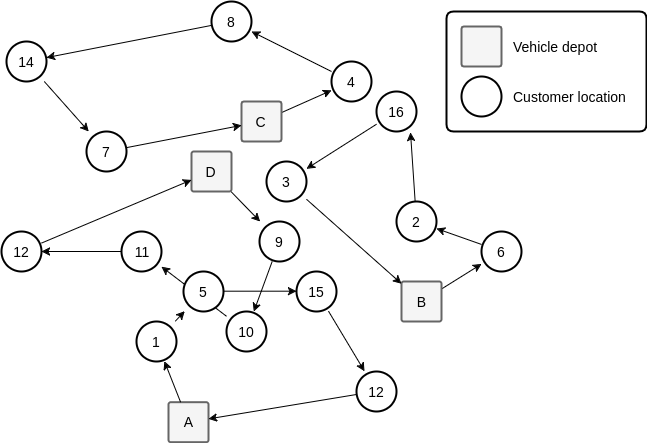
\includegraphics[width=9cm]{Resources/Images/result-mdvrp-illustration}
	\caption{Ilustrasi Rute yang Dihasilkan}
	\label{fig:result-mdvrp-illustration}
\end{figure}


Total \textit{cost} untuk masing-masing rute kemudian dikalkulasi. \textit{Cost} dihitung dalam satuan waktu. Untuk setiap rute, total \textit{cost} tersusun atas penjumlahan seluruh waktu tempuh dan waktu pelayanan (service time) dari lokasi yang dikunjungi. Pada contoh \autoref{fig:result-mdvrp-illustration}, total \textit{cost} dari setiap kendaraan adalah:


\begin{itemize}
	\item $TC_A$ = $C_{A-1}$ + $ST_5$ + $C_{1-5}$ + $ST_5$ + $C_{5-15}$ + $ST_15$ + $C_{15-12}$ + $ST_12$ + $C_{12-A}$
	\item $TC_B$ = $C_{B-6}$ + $ST_6$ + $C_{6-2}$ + $ST_2$ + $C_{2-16}$ + $ST_16$ + $C_{16-3}$ + $ST_3$ + $C_{3-B}$
	\item $TC_C$ = $C_{C-4}$ + $ST_4$ + $C_{4-8}$ + $ST_8$ + $C_{8-14}$ + $ST_14$ + $C_{14-7}$ + $ST_7$ + $C_{7-C}$
	\item $TC_D$ = $C_{D-9}$ + $ST_9$ + $C_{9-10}$ + $ST_10$ + $C_{10-11}$ + $ST_11$ + $C_{11-12}$ + $ST_12$ + $C_{12-D}$
\end{itemize}
dimana TC adalah \textit{total cost}, C adalah \textit{transport cost} yang direpresentasikan dengan waktu tempuh, dan ST adalah \textit{service time}.


\textbf{\textit{Metric}} atau ukuran yang akan digunakan dalam perbandingan adalah standar deviasi dari seluruh rute. Standar deviasi dipilih sebagai ukuran perbandingan karena merepresentasikan kondisi pencacahan yang sebenarnya, dimana semakin kecil variasi waktu dari seluruh pencacah, maka penyelesaian pencacahan akan semakin merata dan penyelesaian pencacahan secara keseluruhan akan lebih cepat. Sistem yang lebih baik akan menghasilkan standar deviasi yang lebih kecil.


%-----------------------------------------------------------------------------%
\subsection{Skenario dan Hasil Pengujian}
%-----------------------------------------------------------------------------%
Untuk memastikan program dapat bekerja dengan baik, selain menggunakan data yang bervariasi, juga akan digunakan berbagai variasi skenario pengujian. \textit{Setup} pengujian dan skenario yang diujicobakan pada penelitian ini beserta hasilnya dijelaskan dibawah ini.


%-----------------------------------------------------------------------------%
\subsubsection{\textit{Message Broker Setup}}
%-----------------------------------------------------------------------------%
Seluruh skenario dalam pengujian ini akan menggunakan Redis sebagai \textit{message broker}. Redis merupakan \textit{in-memory data structure store} yang dapat digunakan sebagai \textit{database}, \textit{cache}, dan \textit{message broker} \citep{redis_introduction_2017}. Redis mempunyai \textit{feature} Redis Cluster, sehingga dapat dengan mudah disusun menjadi \textit{distributed message broker}. Selain itu, Redis \textit{client} tersedia dalam sebagian besar bahasa pemrograman \citep{redis_clients_2017}, sehingga memungkinkan pemilihan bahasa pemrograman dalam implementasi sistem secara lebih fleksibel.


Pada penelitian ini, Redis Cluster dikonfigurasi sebanyak 6 (enam) buah \textit{nodes}, 3 (tiga) node digunakan sebagai \textit{master} dan sisanya sebagai \textit{slave}. Configurasi Redis Cluster pada setiap node sebagaimana terdapat pada \autoref{lst:redis_conf}. Pada konteks Redis, master dapat dianggap sebagai partisi, dan slave dianggap sebagai replikasi dari master. Seluruh node, baik master maupun slave dapat digunakan sebagai \textit{entrypoint}, dimana client terkoneksi.


\begin{listing}[!]
	\caption{Konfigurasi Redis Cluster}
	\label{lst:redis_conf}
	\begin{minted}[showspaces=false,breaklines=true]{java}
cluster-enabled yes
cluster-node-timeout 5000
cluster-config-file nodes.conf
appendonly yes
dir /data
	\end{minted}
\end{listing}


Setelah seluruh Redis \textit{nodes} dikonfigurasi dan dijalankan, maka kemudian \textit{cluster} dapat dibuat dengan menyertakan \textit{nodes} tersebut. Pembuatan \textit{cluster} menggunakan \textit{script} \textbf{redis-trib.rb} yang telah disediakan oleh redis. \textit{Command} yang dieksekusi sebagaimana terdapat pada \autoref{lst:redis_trib_cluster} berikut. Sementara \textit{response} yang diperoleh adalah sebagaimana terdapat pada \autoref{lst:redis_trib_cluster_response}. \autoref{fig:test-flowchart-normal-global-broker} menunjukkan alur Redis Cluster dibuat dan dijalankan.


\begin{listing}[!]
	\caption{Pembuatan Redis Cluster}
	\label{lst:redis_trib_cluster}
	\begin{minted}[showspaces=false,breaklines=true]{java}
/redis-trib.rb create --replicas 1 172.17.0.3 172.17.0.4 172.17.0.5 172.17.0.6 172.17.0.7 172.17.0.8
	\end{minted}
\end{listing}


\begin{listing}[!]
	\caption{Respon Pembuatan Redis Cluster}
	\label{lst:redis_trib_cluster_response}
	\begin{minted}[showspaces=false,breaklines=true]{java}
Creating cluster
Performing hash slots allocation on 6 nodes...
Using 3 masters:
172.17.0.3:6379
172.17.0.4:6379
172.17.0.5:6379
Adding replica 172.17.0.6:6379 to 172.17.0.3:6379
Adding replica 172.17.0.7:6379 to 172.17.0.4:6379
Adding replica 172.17.0.8:6379 to 172.17.0.5:6379
M: 2f0c681921fe52900a6774fb2cc808a8c4e69216 172.17.0.3:6379
slots:0-5460 (5461 slots) master
M: 41a343142847138301ceeb710206284a50bb44a0 172.17.0.4:6379
slots:5461-10922 (5462 slots) master
M: 88ae20b9e75dd5aa58973f13aa89479f52cedfd3 172.17.0.5:6379
slots:10923-16383 (5461 slots) master
S: c5f6764d82ed10793c0c81e54830b4f68b1eacd7 172.17.0.6:6379
replicates 2f0c681921fe52900a6774fb2cc808a8c4e69216
S: 5906f61963d4a5a45478736d976b79db4280b3c7 172.17.0.7:6379
replicates 41a343142847138301ceeb710206284a50bb44a0
S: 635ed817b134b5d14bffd61fe9089867037fee8c 172.17.0.8:6379
replicates 88ae20b9e75dd5aa58973f13aa89479f52cedfd3
Can I set the above configuration? (type 'yes' to accept): yes
Nodes configuration updated
Assign a different config epoch to each node
Sending CLUSTER MEET messages to join the cluster
Waiting for the cluster to join...
Performing Cluster Check (using node 172.17.0.3:6379)
M: 2f0c681921fe52900a6774fb2cc808a8c4e69216 172.17.0.3:6379
slots:0-5460 (5461 slots) master
1 additional replica(s)
M: 88ae20b9e75dd5aa58973f13aa89479f52cedfd3 172.17.0.5:6379
slots:10923-16383 (5461 slots) master
1 additional replica(s)
S: c5f6764d82ed10793c0c81e54830b4f68b1eacd7 172.17.0.6:6379
slots: (0 slots) slave
replicates 2f0c681921fe52900a6774fb2cc808a8c4e69216
M: 41a343142847138301ceeb710206284a50bb44a0 172.17.0.4:6379
slots:5461-10922 (5462 slots) master
1 additional replica(s)
S: 635ed817b134b5d14bffd61fe9089867037fee8c 172.17.0.8:6379
slots: (0 slots) slave
replicates 88ae20b9e75dd5aa58973f13aa89479f52cedfd3
S: 5906f61963d4a5a45478736d976b79db4280b3c7 172.17.0.7:6379
slots: (0 slots) slave
replicates 41a343142847138301ceeb710206284a50bb44a0
[OK] All nodes agree about slots configuration.
Check for open slots...
Check slots coverage...
[OK] All 16384 slots covered.
	\end{minted}
\end{listing}


%-----------------------------------------------------------------------------%
\subsubsection{\textit{Publisher Setup}}
%-----------------------------------------------------------------------------%
Publisher dikonfigurasi dan dijalankan pada lingkungan yang telah didefinisikan pada \autoref{ssec:test-environment}. Publisher dijalankan sesuai dengan alur yang digambarkan pada \autoref{fig:test-flowchart-normal-global-publisher}. \autoref{lst:publisher-usage} menunjukkan format penggunaan dari Publisher.


\begin{listing}[!]
	\caption{Format penggunaan Publisher}
	\label{lst:publisher-usage}
	\begin{minted}[showspaces=false,breaklines=true]{bash}
Usage: mdvrp-redis-producer [options]

Run location recommendation server

Options:
-h, --help            show this help message and exit
-b BIN, --coes-bin=BIN
Binary of CoES MDVRP library
-D D, --data=D        Data problem file
-C C, --cost-file=C   Cost matrix file
-O O, --output-dir=O  Output directory
-t, --use-timestamp   Append timestamp to output directory
-B B, --broker-url=B  Redis broker URL
-X X, --solver-execution-time=X
VRP Solver execution time
	\end{minted}
\end{listing}


%-----------------------------------------------------------------------------%
\subsubsection{\textit{Subscriber Setup}}
%-----------------------------------------------------------------------------%
Pada masing-masing pengujian juga dibuat sebuah program tambahan yang berperan sebagai pencacah. Seluruh pencacah akan berperan sebagai subscriber. Alur kerja dari masing-masing \textit{subscriber}, sebagaimana digambarkan pada \autoref{fig:test-flowchart-normal-global-subscriber} adalah sebagai berikut:


\begin{enumerate}
	\item Lakukan \textit{subscription} pada \textit{message broker} dengan topik \textit{current location}, 
	\item Sebuah pesan akan diterima, dimana pesan dari \textit{publisher} yang di\textit{publish} melalui \textit{message broker} menunjukkan lokasi berikutnya yang akan dikunjungi,
	\item Simulasikan perjalanan ke lokasi yang akan dikunjungi dengan \textit{delay},
	\item Setelah sampai ke lokasi, maka simpan \textit{current location} pada \textit{shared memory}, 
	\item Simulasikan pencacahan dengan \textit{delay}, 
	\item Ulangi lagi dari langkah pertama.
\end{enumerate}


\begin{figure}[!]
	\centering
	\begin{subfigure}[t]{0.3\textwidth}
		\centering
		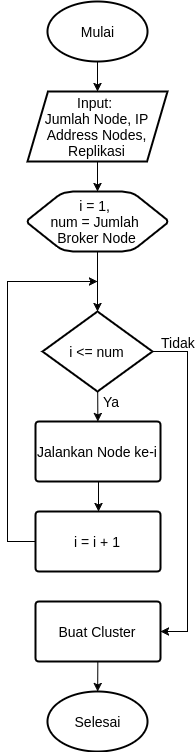
\includegraphics[width=\textwidth]{Resources/Images/test-flowchart-normal-global-broker}
		\caption{\textit{Flowchart Message Broker}}
		\label{fig:test-flowchart-normal-global-broker}
	\end{subfigure}%
	~
	\begin{subfigure}[t]{0.39\textwidth}
		\centering
		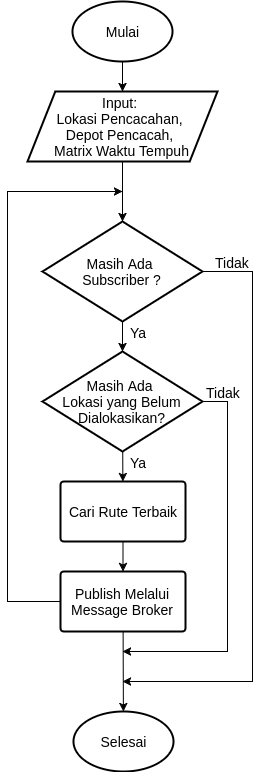
\includegraphics[width=\textwidth]{Resources/Images/test-flowchart-normal-global-publisher}
		\caption{\textit{Flowchart Publisher}}
		\label{fig:test-flowchart-normal-global-publisher}
	\end{subfigure}%
	~
	\begin{subfigure}[t]{0.31\textwidth}
		\centering
		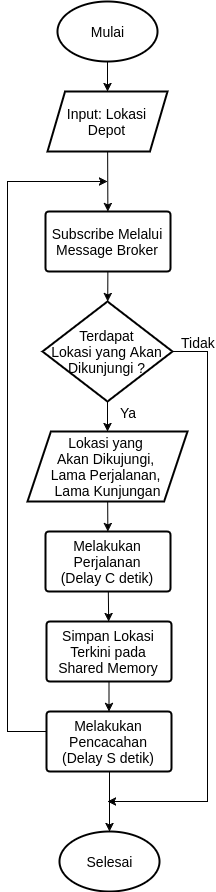
\includegraphics[width=\textwidth]{Resources/Images/test-flowchart-normal-global-subscriber}
		\caption{\textit{Flowchart Subscriber}}
		\label{fig:test-flowchart-normal-global-subscriber}
	\end{subfigure}
	\caption{\textit{Flowchart} Subsistem pada Pengujian}
	\label{fig:test-flowchart-normal-global}
\end{figure}


%-----------------------------------------------------------------------------%
\subsubsection{Pengujian Tanpa \textit{Service Time}}
%-----------------------------------------------------------------------------%
Pengujian ini bertujuan membandingkan keakuratan sistem dalam memproses data yang tidak memasukkan \textit{service time} pada \textit{customer}nya. Pada pengujian ini digunakan data dimana kendaraan dan \textit{customer} digenerate secara random, baik secara jumlah maupun koordinat. Data yang digunakan diperoleh dari \textit{instance} Cordeau P01 sampai P10.


Dari hasil simulasi, diperoleh rute untuk masing-masing \textit{instance} Cordeau sebagaimana digambarkan pada \hyperref[ch:test_result_cordeau_notw]{Lampiran 1}. Kemudian dari seluruh rute yang diperoleh, dikalkulasi \textit{total time} untuk masing-masing rute, sebagaimana cara yang dijelaskan pada \autoref{sssec:metric}. Berdasarkan \autoref{tbl:test_result_10_cordeau}, diperoleh hasil bahwasannya dengan menggunakan sistem usulan hanya 2 dari 10 \textit{instance} menghasilkan \textbf{total waktu} yang lebih kecil. Sementara dari sisi \textbf{standar deviasi}, diperoleh hasil 8 dari 10 \textit{instance} menghasilkan standar deviasi yang lebih kecil. Hal ini berarti, program pembanding, yaitu MDVRP berbasis CoEAs, lebih efisien, tetapi program usulan, yaitu MDVRP berbasis CoEAs yang dikombinasikan dengan mekanisme Publish/Subscribe lebih merata. \autoref{fig:test_result_10_cordeau_total_time} dan \autoref{fig:test_result_10_cordeau_standard_deviation} menggambarkan perbandingan hasil pengujian dari 10 \textit{instance} Cordeau.


\newcommand\MyHead[2]{%
	\multicolumn{1}{l}{\parbox{#1}{\centering #2}}
}


\begin{longtable}[!]{l|rrrr}
	\caption{Hasil Pengujian Tanpa \textit{Service Time} pada Data Cordeau}
	\label{tbl:test_result_10_cordeau}\\
	\toprule
	\textit{Instance} & \MyHead{2.5cm}{Total CoES MDVRP} & \MyHead{2.5cm}{Total CoES MDVRP + Pub/Sub} & \MyHead{2.5cm}{Stdev CoES MDVRP} & \MyHead{2.5cm}{Stdev CoES MDVRP + Pub/Sub} \\ 
	\midrule
	\endfirsthead
	\toprule
	\textit{Instance} & \MyHead{2.5cm}{Total CoES MDVRP} & \MyHead{2.5cm}{Total CoES MDVRP + Pub/Sub} & \MyHead{2.5cm}{Stdev CoES MDVRP} & \MyHead{2.5cm}{Stdev CoES MDVRP + Pub/Sub} \\ 
	\midrule
	\endhead
	\bottomrule
	\endfoot
	p01 & \textbf{454.91} & 573.77 & 27.24 & \textbf{20.84} \\
	p02 & \textbf{462.61} & 550.61 & 25.90 & \textbf{13.32} \\
	p03 & \textbf{590.98} & 696.93 & 32.47 & \textbf{20.09} \\
	p04 & 1.321.89 & \textbf{1.264.53} & 199.16 & \textbf{16.10} \\
	p05 & \textbf{1.039.68} & 1.520.53 & 76.61 & \textbf{1.09} \\
	p06 & \textbf{679.11} & 1.160.76 & 57.15 & \textbf{48.82} \\
	p07 & \textbf{782.41} & 973.72 & \textbf{29.08} & 67.27 \\
	p08 & 8.353.76 & \textbf{6.172.66} & 1.962.81 & \textbf{228.95} \\
	p09 & \textbf{2.669.29} & 4.275.12 & 208.99 & \textbf{117.76} \\
	p10 & \textbf{2.692.06} & 4.132.31 & \textbf{130.08} & 200.31 \\
\end{longtable}


\begin{figure}[H]
	\centering
	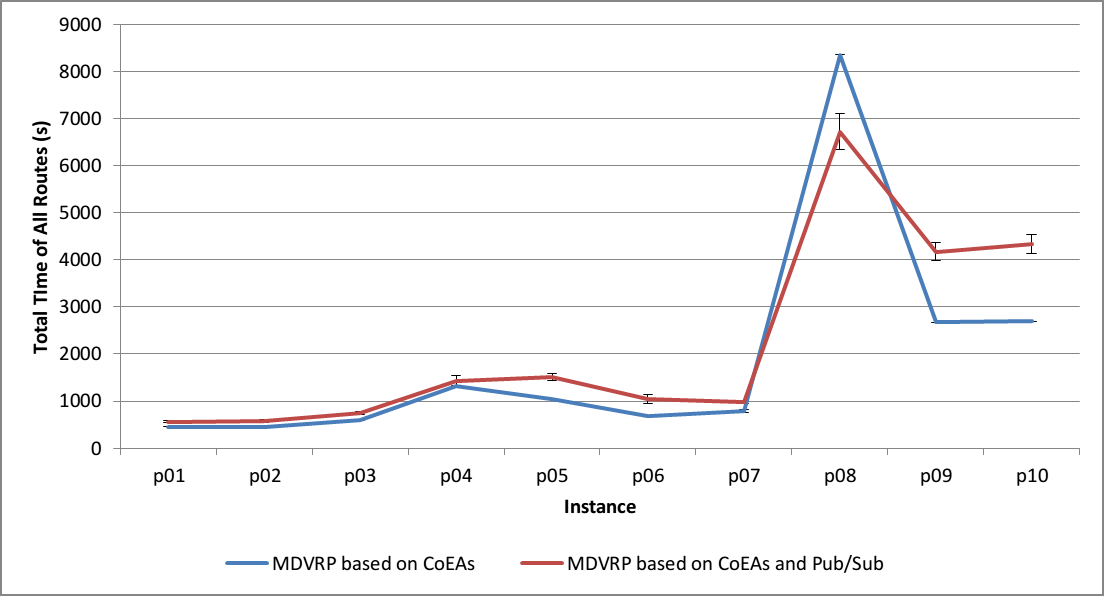
\includegraphics[width=\textwidth]{Resources/Images/test_result_10_cordeau_total_time}
	\caption{Perbandingan Waktu Total dari 10 \textit{Instance} Cordeau}
	\label{fig:test_result_10_cordeau_total_time}
\end{figure}


\begin{figure}[H]
	\centering
	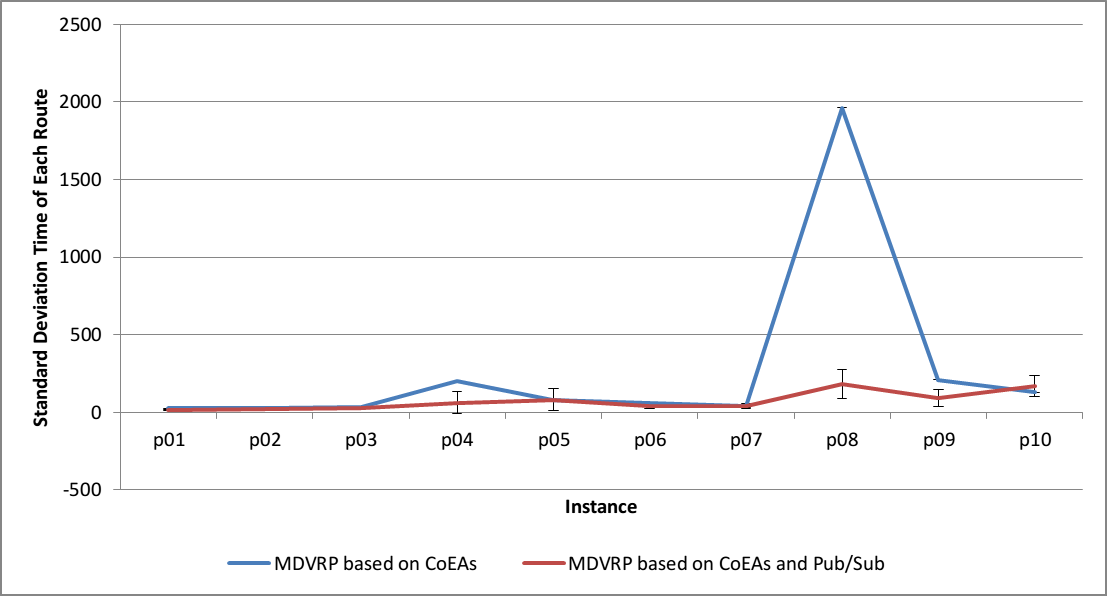
\includegraphics[width=\textwidth]{Resources/Images/test_result_10_cordeau_standard_deviation}
	\caption{Perbandingan Standar Deviasi Waktu dari 10 \textit{Instance} Cordeau}
	\label{fig:test_result_10_cordeau_standard_deviation}
\end{figure}


%-----------------------------------------------------------------------------%
\subsubsection{Pengujian Kondisi Normal dengan \textit{Service Time}}
\label{ssec:test-normal-service-time}
%-----------------------------------------------------------------------------%
Skenario pengujian kondisi normal dimaksudkan untuk membandingkan sistem yang dijalankan pada kondisi normal. Yang dimaksud kondisi normal disini merupakan kondisi dimana tidak ada yang menyebabkan penundaaan, seperti permasalahan koneksi. Pengujian kondisi ini akan dilakukan satu kali untuk masing-masing data set, Cordeau P01 dan data lapangan.


Sementara data \textit{service time} digenerate secara random dengan mengikuti komposisi dari \citep{sudman_time_1965}, yaitu:
\begin{enumerate}
	\item 21 persen dari total waktu untuk perpindahan antar segmen, 
	\item 15 persen dari total waktu untuk perpindahan antar rumah tangga dalam segmen, 
	\item 37 persen dari total waktu untuk wawancara seluruh responden, dan 
	\item 27 persen untuk hal-hal yang lain, seperti pengenalan wilayah dan perbaikan data.
\end{enumerate}
\textit{Service time} merupakan gabungan dari waktu perpindahan antar rumah tangga dan waktu wawancara.


Setelah simulasi dilakukan, dari seluruh rute yang diperoleh kemudian dikalkulasi \textit{total time} untuk masing-masing rute, sebagaimana cara yang dijelaskan pada \autoref{sssec:metric}. Selain itu juga sebuah grafik dibuat untuk memberikan ilustrasi rute pada masing-masing program pembanding dan sistem usulan.


Pada pengujian dengan dataset Cordeau, diperoleh hasil sebagaimana \autoref{tbl:test_result_normal_cordeau_coes} untuk algoritma MDVRP berbasis CoEAs tanpa mekanisme Publish/Subscribe, dan \autoref{tbl:test_result_normal_cordeau_pubsub_coes} untuk algoritma MDVRP berbasis CoEAs dengan mekanisme Publish/Subscribe. Sementara \autoref{fig:test_result_normal_cordeau_comparison} menggambarkan rute yang diperoleh untuk masing-masing program.


Berdasarkan \autoref{tbl:test_result_normal_cordeau_comparison}, diperoleh hasil bahwasannya \textbf{total waktu} yang diperoleh dengan menggunakan sistem MDVRP berbasis CoEAs dan Publish/Subscribe lebih buruk 6,25 persen  dibandingkan dengan program usulan. Akan tetapi dari sisi \textbf{standar deviasi} dari keseluruhan rute diperoleh hasil metode CoEAs yang dikombinasikan dengan Publish/Subscribe menghasilkan angka yang lebih baik 68.83 persen, yang artinya total waktu dari seluruh rute lebih merata.


\begin{longtable}[!]{lp{8cm}r}
	\caption{Hasil Pengujian Kondisi Normal (Cordeau), MDVRP berbasis CoEAs}
	\label{tbl:test_result_normal_cordeau_coes}\\
	\toprule
		\textit{Vehicle} & Rute & Waktu Total\\ 
	\midrule
	\endfirsthead
	\toprule
		\textit{Vehicle} & Rute & Waktu Total\\ 
	\midrule
	\endhead
	\bottomrule
	\endfoot
		51 & 42-19-40-41-13-18-4-17-37-15-44 & 194,775.99 \\
		52 & 27-48-6-14-25-24-43-23-7-26-8-1-32-11-12-47-46 & 312,308.79 \\
		53 & 9-38-5-45-33-39-10-30-34-50-49 & 198,178.68 \\
		54 & 29-21-16-2-22-28-31-3-20-35-36 & 199,754.93 \\
\end{longtable}


\begin{longtable}[!]{lp{8cm}r}
	\caption{Hasil Pengujian Kondisi Normal (Cordeau), MDVRP berbasis CoEAs dan Publish/Subscribe}
	\label{tbl:test_result_normal_cordeau_pubsub_coes}\\
	\toprule
		\textit{Vehicle} & Rute & Waktu Total\\ 
	\midrule
	\endfirsthead
	\toprule
		\textit{Vehicle} & Rute & Waktu Total\\ 
	\midrule
	\endhead
	\bottomrule
	\endfoot
		51 & 42-19-44-40-45-33-15-37-39-30-17-25-43 & 234,931.69 \\
		52 & 27-46-12-47-18-24-4-41-6-48-13-14-23 & 236,669.22 \\
		53 & 9-50-34-49-5-10-38-11-16-2-32 & 199,526.52 \\
		54 & 29-21-20-35-36-31-28-3-22-26-1-8-7 & 234,154.12 \\
\end{longtable}


\begin{longtable}[!]{lrr}
	\caption{Komparasi Hasi Pengujian Kondisi Normal Dengan Data Cordeau}
	\label{tbl:test_result_normal_cordeau_comparison}\\
	\toprule
		\textit{Parameter} & CoEAs MDVRP  & Pub/Sub CoEAS MDVRP\\ 
	\midrule
	\endfirsthead
	\toprule
		\textit{Parameter} & CoEAs MDVRP  & Pub/Sub CoEAS MDVRP\\ 
	\midrule
	\endhead
	\bottomrule
	\endfoot
		Total Waktu & \textbf{905,018.39} & 905,281.55\\
		Rata-rata & \textbf{226,254.60} & 226,320.39\\
		Standar Deviasi & 49,715.99 & \textbf{15,496.22}\\
\end{longtable}


\begin{figure}[!]
    \centering
    \begin{subfigure}[t]{\textwidth}
        \centering
		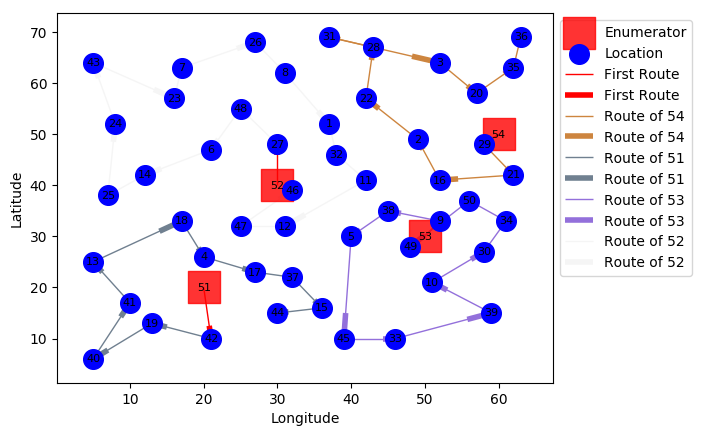
\includegraphics[width=\textwidth]{Resources/Images/test_result_normal_cordeau_p01_coes}
		\caption{MDVRP berbasis CoEAs}
		\label{fig:test_result_normal_cordeau_coes}
    \end{subfigure}%
    
    \begin{subfigure}[t]{\textwidth}
        \centering
		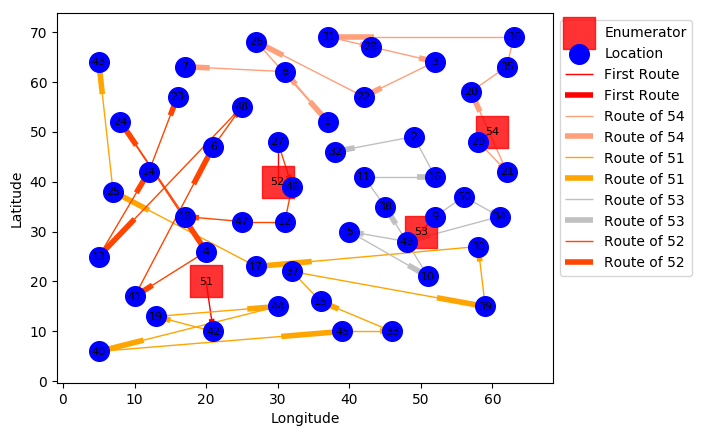
\includegraphics[width=\textwidth]{Resources/Images/test_result_normal_cordeau_p01_pubsub_coes}
		\caption{MDVRP berbasis CoEAs dengan Publish/Subscribe}
		\label{fig:test_result_normal_cordeau_pubsub_coes}
    \end{subfigure}
    \caption{Perbandingan Rute Hasil Pengujian Data Cordeau P01 Dengan \textit{Service Time}}
    \label{fig:test_result_normal_cordeau_comparison}
\end{figure}


Sementara itu, pada pengujian dengan menggunakan data lapangan, diperoleh hasil sebagaimana \autoref{tbl:test_result_normal_field_coes} untuk algoritma MDVRP berbasis CoEAs tanpa mekanisme Publish/Subscribe, dan \autoref{tbl:test_result_normal_field_pubsub_coes} untuk algoritma MDVRP berbasis CoEAs dengan mekanisme Publish/Subscribe. Sementara \autoref{fig:test_result_normal_field_comparison} menggambarkan rute yang diperoleh untuk masing-masing program.


Berdasarkan \autoref{tbl:test_result_normal_field_comparison}, diperoleh hasil bahwasannya \textbf{total waktu} yang diperoleh dengan menggunakan sistem MDVRP berbasis CoEAs dan Publish/Subscribe lebih buruk 8,25 persen  dibandingkan dengan program usulan. Akan tetapi dari sisi \textbf{standar deviasi} dari keseluruhan rute diperoleh hasil metode CoEAs yang dikombinasikan dengan Publish/Subscribe menghasilkan angka yang lebih baik 59,11 persen, yang artinya total waktu dari seluruh rute lebih merata.


\begin{longtable}[!]{lp{8cm}r}
	\caption{Hasil Pengujian Kondisi Normal (Lapangan), MDVRP berbasis CoEAs}
	\label{tbl:test_result_normal_field_coes}\\
	\toprule
		\textit{Vehicle} & Rute & Waktu Total\\ 
	\midrule
	\endfirsthead
	\toprule
		\textit{Vehicle} & Rute & Waktu Total\\ 
	\midrule
	\endhead
	\bottomrule
	\endfoot
		183 & 70-179-87-163-132-5-35-145-42 & 170,349.48 \\
		184 & 159-174-60-36-99-98-171-50-9-7-8-152-111-51-40-172-38-134 & 331,759.24 \\
		185 & 127-88-147-173-158-102-124-37-73-97 & 184,993.17 \\
		186 & 157-93-94-146-155-123-162-161-156-89-138-77-44-109 & 254,089.65 \\
		187 & 149-135-61-115-180-128 & 109,758.28 \\
		188 & 165-47-92-78-69-108-120-136-41-71-55-4-33-178-160-1-151-3-2 & 355,614.60 \\
		189 & 13-91-10-11-14-12-118-167-176 & 168,298.11 \\
		190 & 104-141-63-117-45-131-81-177-170-67-49 & 193,952.81 \\
		191 & 100-107-116-150-32-59 & 116,272.15 \\
		192 & 86-168-143-95-76-103-53-52-166-65-54 & 211,842.84 \\
		193 & 164-139-56-18-72-19-20-22-21-16-39-24-23-17-28-137-26-169-154-27-15-25-122-31 & 451,562.34 \\
		194 & 142-126-30-58-110-46-82-80-148-106-96-84-68-182-34 & 275,108.47 \\
		195 & 83-140-175-79-64-133-119-66-48 & 160,970.13 \\
		196 & 29-112-113-43-121-74-90-125-153-6-181-62 & 220,804.42 \\
		197 & 85-129-130-105-114-57-144-75-101 & 168,014.48 \\
\end{longtable}


\begin{longtable}[!]{lp{8cm}r}
	\caption{Hasil Pengujian Kondisi Normal (Lapangan), MDVRP berbasis CoEAs dan Publish/Subscribe}
	\label{tbl:test_result_normal_field_pubsub_coes}\\
	\toprule
		\textit{Vehicle} & Rute & Waktu Total\\ 
	\midrule
	\endfirsthead
	\toprule
		\textit{Vehicle} & Rute & Waktu Total\\ 
	\midrule
	\endhead
	\bottomrule
	\endfoot
		183 & 70-179-87-163-132-38-51-68-96-139-58-7-30-8 & 277,856.33 \\
		184 & 159-36-174-40-60-172-102-178-49-3-177-151 & 241,245.62 \\
		185 & 127-88-147-173-158-1-124-37-67-73-170-97-77 & 253,954.73 \\
		186 & 157-109-93-156-44-155-89-123-161-115-180-128-48-65-162 & 280,828.06 \\
		187 & 149-135-61-94-146-138-120-136-12-71-176-33 & 269,049.32 \\
		188 & 165-41-47-69-78-81-108-116-92-55-4-160-2 & 257,633.11 \\
		189 & 13-91-10-11-131-167-118-14-126-110-148 & 229,909.92 \\
		190 & 104-141-117-45-63-150-103-53-133-54-52-166 & 242,338.23 \\
		191 & 100-107-32-59-76-64-66-171-119-9 & 246,133.18 \\
		192 & 86-168-143-95-84-152-98-122-50-31-134-56-28 & 275,294.42 \\
		193 & 164-24-182-106-111-99-39-22-72-21-19-16-20 & 258,783.38 \\
		194 & 142-34-46-80-82-23-26-169-27-15-137-25-154-18-17 & 284,033.04 \\
		195 & 83-140-175-79-121-75-43-5-125-153-6 & 220,121.19 \\
		196 & 29-112-74-62-129-114-144 & 132,181.37 \\
		197 & 85-130-101-57-105-113-181-35-90-42-145 & 207,356.29 \\
\end{longtable}


\begin{longtable}[!]{lrr}
	\caption{Komparasi Hasi Pengujian Kondisi Normal Dengan Data Lapangan}
	\label{tbl:test_result_normal_field_comparison}\\
	\toprule
	\textit{Parameter} & CoEAs MDVRP  & Pub/Sub CoEAS MDVRP\\ 
	\midrule
	\endfirsthead
	\toprule
	\textit{Parameter} & CoEAs MDVRP  & Pub/Sub CoEAS MDVRP\\ 
	\midrule
	\endhead
	\bottomrule
	\endfoot
		Total Waktu & \textbf{3,373,390.19} & 3,676,718.19\\
		Rata-rata & \textbf{224,892.68} & 245,114.55\\
		Standar Deviasi & 91,123.23 & \textbf{37,261.85}\\
\end{longtable}


\begin{figure}[H]
	\centering
	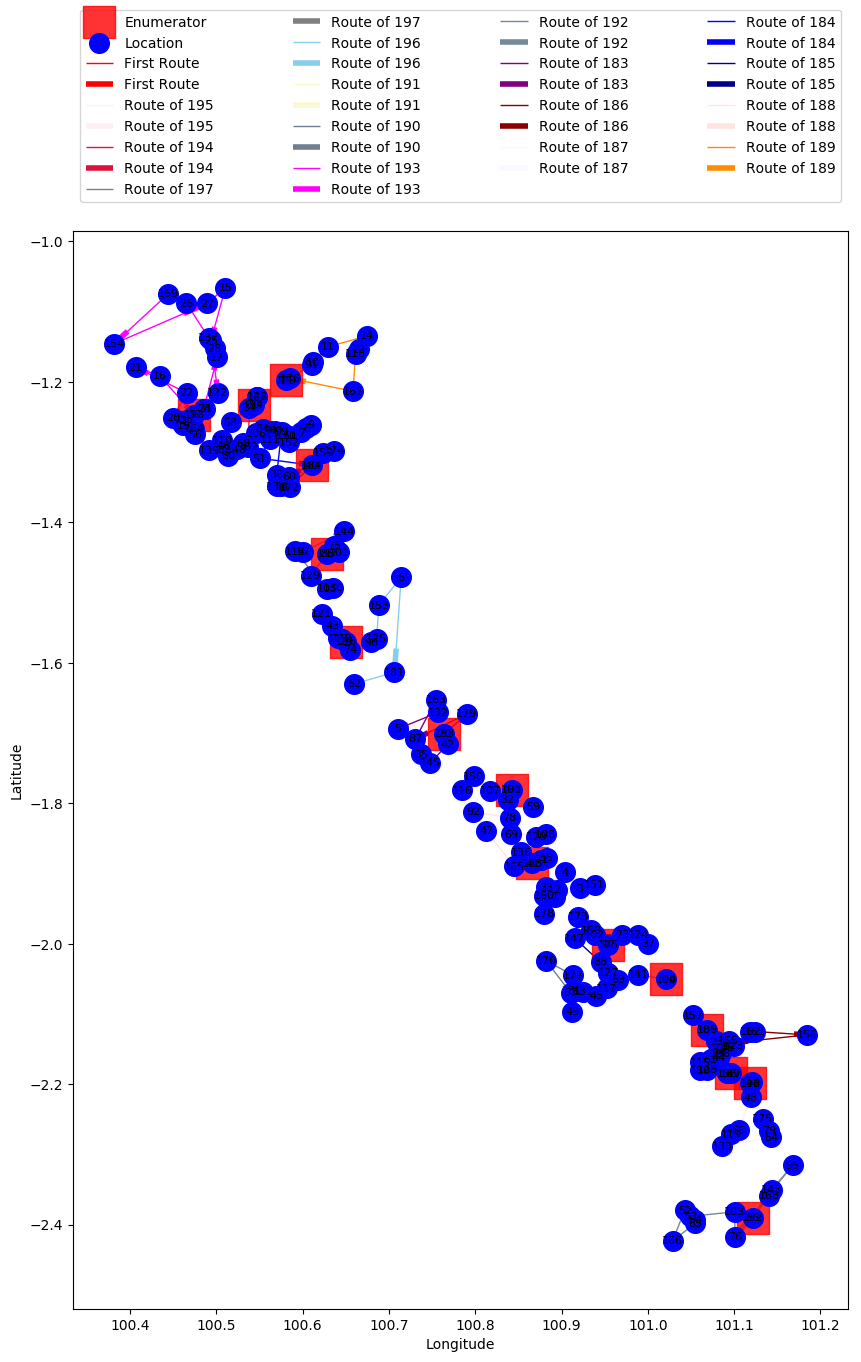
\includegraphics[width=\textwidth]{Resources/Images/test_result_normal_field_m15_n182_coes}
	\caption{Rute Hasil Pengujian Data Lapangan Pada MDVRP berbasis CoEAs}
	\label{fig:test_result_normal_field_coes}
\end{figure}


\begin{figure}[H]
	\centering
	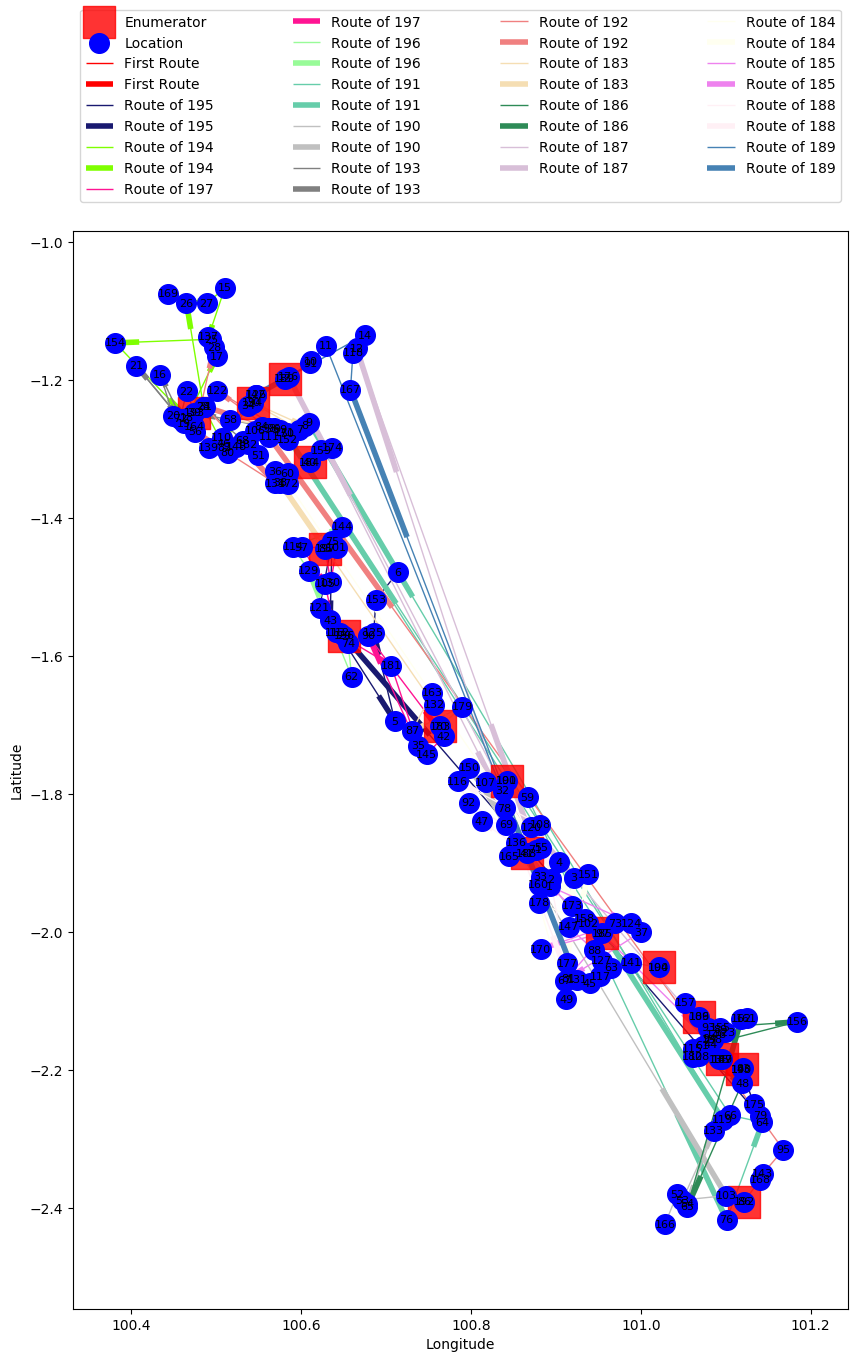
\includegraphics[width=\textwidth]{Resources/Images/test_result_normal_field_m15_n182_pubsub_coes}
	\caption{Rute Hasil Pengujian Data Lapangan Pada MDVRP berbasis CoEAs dengan Publish/Subscribe}
	\label{fig:test_result_normal_field_pubsub_coes}
\end{figure}


%-----------------------------------------------------------------------------%
\subsubsection{Pengujian Kondisi \textit{Delay} pada Jaringan dengan \textit{Service Time}}
%-----------------------------------------------------------------------------%
Skenario pengujian kondisi \textit{delay} pada jaringan dimaksudkan untuk membandingkan program yang dijalankan pada kondisi dimana terjadi \textit{delay} secara random. Pengujian ini digunakan sebagai cerminan kodisi lapangan dimana pada beberapa lokasi tidak terdapat koneksi yang stabil. Pengujian akan dilakukan satu kali untuk data lapangan. Sementara data \textit{service time} digenerate secara random dengan mengikuti komposisi dari \citep{sudman_time_1965} sebagaimana dijelaskan pada \autoref{ssec:test-normal-service-time}.


Pada pengujian ini akan digunakan sebuah software \textit{$3^{rd}$}, yaitu Pumba \citep{1013821358660176_pumba_2016} untuk meng-emulasi-kan \textit{delay}. \textit{Delay} yang digunakan adalah 100ms $\pm$ 10\% pada setiap koneksi yang terjadi. Langkah-langkah yang dilakukan dalam konfigurasi Pumba adalah seperti pada \autoref{fig:test-flowchart-normal-global-netem}.


\begin{figure}[!]
	\centering
	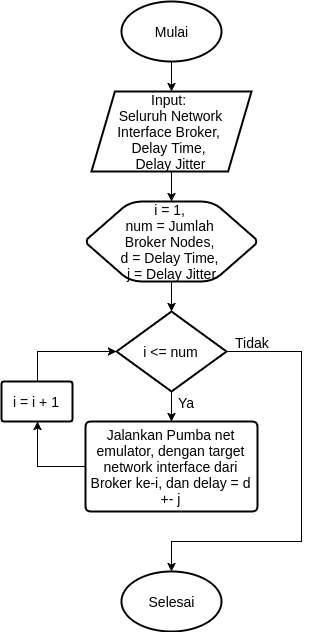
\includegraphics[width=0.5\textwidth]{Resources/Images/test-flowchart-normal-global-netem}
	\caption{Flowchart Setup Pumba Net Emulator}
	\label{fig:test-flowchart-normal-global-netem}
\end{figure}


Berdasarkan hasil pengujian, diperoleh hasil sebagaimana \autoref{tbl:test_result_network_delay_field_coes} untuk algoritma MDVRP berbasis CoEAs tanpa mekanisme Publish/Subscribe, dan \autoref{tbl:test_result_network_delay_field_pubsub_coes} untuk algoritma MDVRP berbasis CoEAs dengan mekanisme Publish/Subscribe. Sementara \autoref{fig:test_result_network_delay_field_comparison} menggambarkan rute yang diperoleh untuk masing-masing program.


Berdasarkan \autoref{tbl:test_result_network_delay_field_comparison}, diperoleh hasil bahwasannya \textbf{total waktu} yang diperoleh dengan menggunakan sistem MDVRP berbasis CoEAs dan Publish/Subscribe lebih buruk 4,83 persen  dibandingkan dengan program usulan. Akan tetapi dari sisi \textbf{standar deviasi} dari keseluruhan rute diperoleh hasil metode CoEAs yang dikombinasikan dengan Publish/Subscribe menghasilkan angka yang lebih baik 3,62 persen, yang artinya total waktu dari seluruh rute lebih merata.


\begin{longtable}[!]{lp{8cm}r}
	\caption{Hasil Pengujian Kondisi Network Delay, MDVRP berbasis CoEAs}
	\label{tbl:test_result_network_delay_field_coes}\\
	\toprule
	\textit{Vehicle} & Rute & Waktu Total\\ 
	\midrule
	\endfirsthead
	\toprule
	\textit{Vehicle} & Rute & Waktu Total\\ 
	\midrule
	\endhead
	\bottomrule
	\endfoot
	183 & 70-179-87-163-132-5-35-145-42 & 170,349.48 \\
	184 & 172-38-134-60-36-99-98-171-50-9-7-8-152-111-51-40-159-174 & 330,854.24 \\
	185 & 127-88-147-173-158-102-124-37-73-97 & 184,993.17 \\
	186 & 109-157-93-94-146-155-123-162-161-156-89-138-77-44 & 253,318.65 \\
	187 & 149-135-61-115-180-128 & 109,758.28 \\
	188 & 41-71-55-4-33-178-160-1-151-3-2-165-47-92-78-69-108-120-136 & 355,930.60 \\
	189 & 13-91-10-11-14-12-118-167-176 & 168,298.11 \\
	190 & 104-141-63-117-45-131-81-177-170-67-49 & 193,952.81 \\
	191 & 100-107-116-150-32-59 & 116,272.15 \\
	192 & 86-168-143-95-76-103-53-52-166-65-54 & 211,842.84 \\
	193 & 24-23-17-28-137-26-169-154-27-15-25-122-31-164-139-56-18-72-19-20-22-21-16-39 & 451,654.34 \\
	194 & 30-58-110-46-82-80-148-106-96-84-68-182-34-142-126 & 275,108.47 \\
	195 & 83-140-175-79-64-133-119-66-48 & 160,970.13 \\
	196 & 29-112-113-43-121-74-90-125-153-6-181-62 & 220,804.42 \\
	197 & 85-129-130-105-114-57-144-75-101 & 168,014.48 \\
\end{longtable}


\begin{longtable}[!]{lp{8cm}r}
	\caption{Hasil Pengujian Kondisi Network Delay, MDVRP berbasis CoEAs dan Publish/Subscribe}
	\label{tbl:test_result_network_delay_field_pubsub_coes}\\
	\toprule
	\textit{Vehicle} & Rute & Waktu Total\\ 
	\midrule
	\endfirsthead
	\toprule
	\textit{Vehicle} & Rute & Waktu Total\\ 
	\midrule
	\endhead
	\bottomrule
	\endfoot
	183 & 70-179-87-132-163-125-90-181 & 151,466.36 \\
	184 & 172-38-60-99-134-98-152-171-111-50-174-9-80-96-176-36-12-40-11 & 377,075.90 \\
	185 & 127-88-117-147-173-158-178-1-160-102-2-33 & 225,310.18 \\
	186 & 109-93-157-146-89-123-155-162-156-161 & 181,632.75 \\
	187 & 149-135-61-115-180-128-48-94-138-77-44 & 201,434.48 \\
	188 & 41-165-71-4-136-55-120-59-63-124-73 & 210,047.14 \\
	189 & 13-91-92-32-69-47-78-108 & 159,479.98 \\
	190 & 104-141-49-170-67-177-81-131-45-97-37-151-3 & 240,785.25 \\
	191 & 100-107-116-150-145-5-35-42 & 148,534.65 \\
	192 & 86-168-143-95-76-103-53-54-16-166-19-139-164-68-46-159-39 & 389,335.84 \\
	193 & 24-31-17-28-137-26-22-169-21-27-154-15-72-25-18-122-20-23-56-82 & 394,523.78 \\
	194 & 30-34-110-142-58-126-182-106-51-84-148-118-8-10-7-167-14 & 334,526.44 \\
	195 & 83-140-175-79-64-66-133-119-52-65 & 183,551.19 \\
	196 & 29-112-113-43-121-74-62-153-144-6 & 194,797.02 \\
	197 & 85-101-57-129-130-105-114-75 & 150,698.22 \\
\end{longtable}


\begin{longtable}[!]{lrr}
	\caption{Komparasi Hasil Pengujian Kondisi Network Delay Dengan Data Lapangan}
	\label{tbl:test_result_network_delay_field_comparison}\\
	\toprule
	\textit{Parameter} & CoEAs MDVRP  & Pub/Sub CoEAS MDVRP\\ 
	\midrule
	\endfirsthead
	\toprule
	\textit{Parameter} & CoEAs MDVRP  & Pub/Sub CoEAS MDVRP\\ 
	\midrule
	\endhead
	\bottomrule
	\endfoot
	Total Waktu & \textbf{3,372,122.19} & 3,543,199.19\\
	Rata-rata & \textbf{224,808.15} & 236,213.28\\
	Standar Deviasi & 91,081.99 & \textbf{87,783.27}\\
\end{longtable}


\begin{figure}[H]
	\centering
	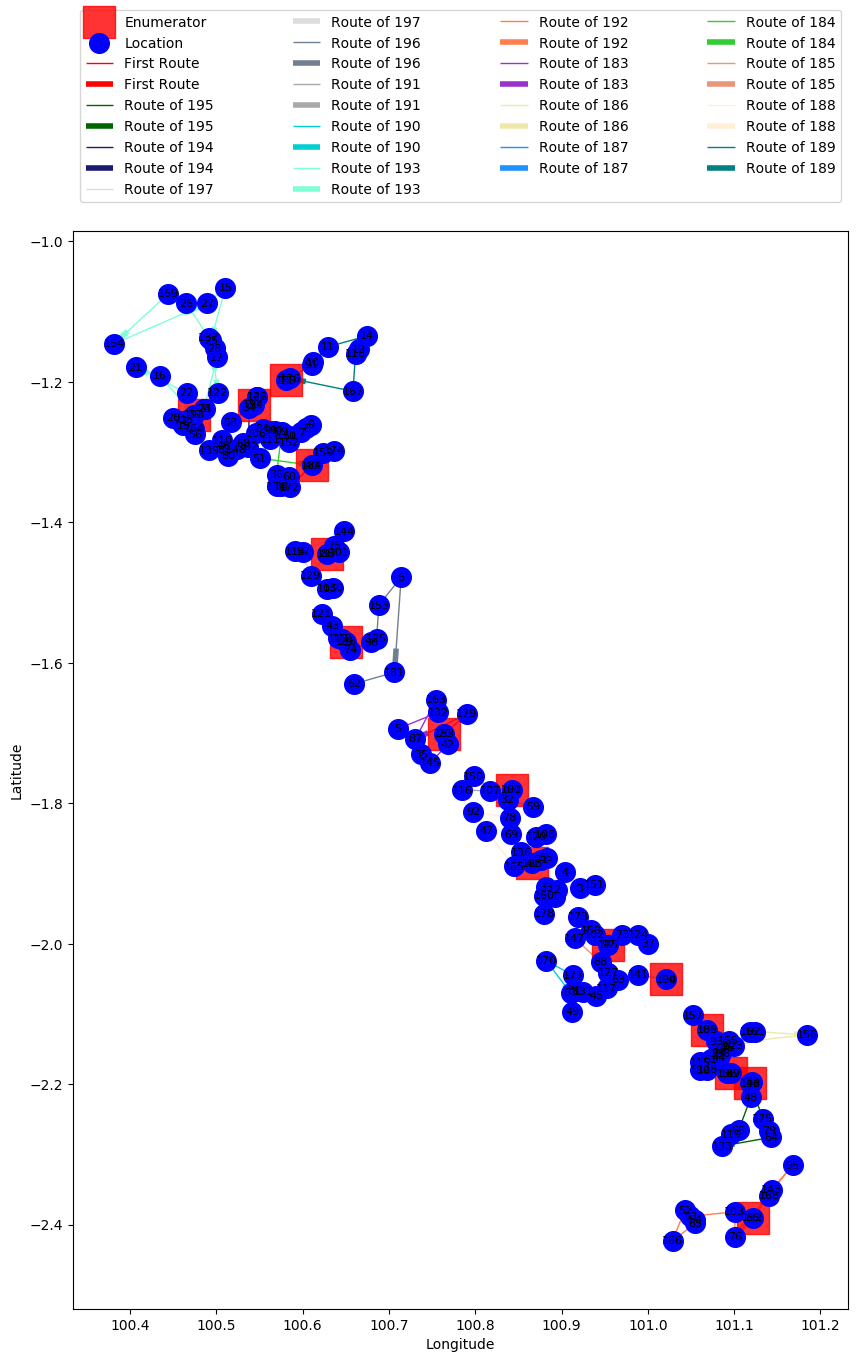
\includegraphics[width=\textwidth]{Resources/Images/test_result_normal_field_m15_n182_delay_coes}
	\caption{Rute Hasil Pengujian Kondisi \textit{Network Delay} Data Lapangan Pada MDVRP berbasis CoEAs}
	\label{fig:test_result_network_delay_field_coes}
\end{figure}


\begin{figure}[H]
	\centering
	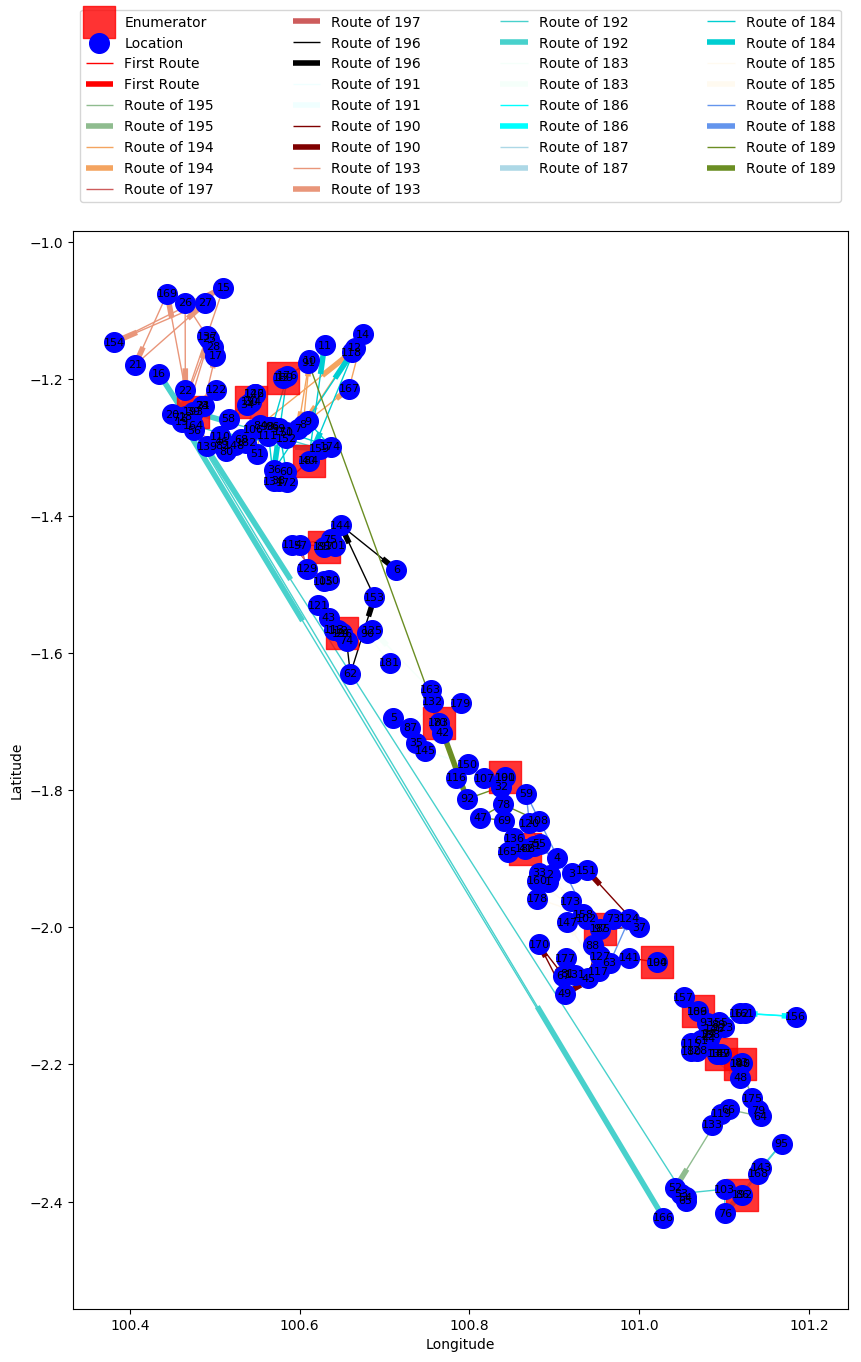
\includegraphics[width=\textwidth]{Resources/Images/test_result_normal_field_m15_n182_delay_pubsub_coes}
	\caption{Rute Hasil Pengujian Kondisi \textit{Network Delay} Data Lapangan Pada MDVRP berbasis CoEAs dengan Publish/Subscribe}
	\label{fig:test_result_network_delay_field_comparison}
\end{figure}


%-----------------------------------------------------------------------------%
\subsubsection{Pengujian Kondisi \textit{Packet Loss} pada Jaringan dengan \textit{Service Time}}
%-----------------------------------------------------------------------------%
Skenario pengujian kondisi \textit{packet loss} pada jaringan dimaksudkan untuk membandingkan program yang dijalankan pada kondisi dimana terjadi \textit{packet loss}. Pengujian ini digunakan sebagai cerminan kodisi lapangan dimana pada beberapa lokasi tidak terdapat koneksi yang stabil. Pengujian akan dilakukan satu kali untuk data lapangan. Sementara data \textit{service time} digenerate secara random dengan mengikuti komposisi dari \citep{sudman_time_1965} sebagaimana dijelaskan pada \autoref{ssec:test-normal-service-time}.


Pada pengujian ini juga akan digunakan sebuah software \textit{$3^{rd}$}, yaitu Pumba \citep{1013821358660176_pumba_2016} untuk meng-emulasi-kan \textit{packet loss}. Nilai \textit{Packet loss} yang digunakan adalah 10\% dari packet yang lewat yang dipilih secara random. Langkah-langkah yang dilakukan dalam konfigurasi Pumba adalah seperti pada \autoref{fig:test-flowchart-normal-global-netem}.


\begin{figure}[!]
	\centering
	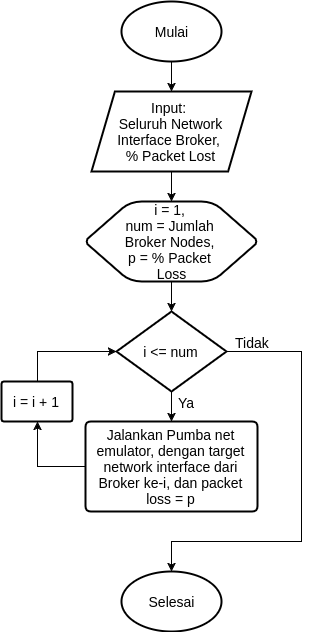
\includegraphics[width=0.5\textwidth]{Resources/Images/test-flowchart-normal-global-netem-packet-loss}
	\caption{Flowchart Setup Pumba Net Emulator}
	\label{fig:test-flowchart-normal-global-netem-packet-loss}
\end{figure}


Berdasarkan hasil pengujian, diperoleh hasil sebagaimana \autoref{tbl:test_result_packet_loss_field_coes} untuk algoritma MDVRP berbasis CoEAs tanpa mekanisme Publish/Subscribe, dan \autoref{tbl:test_result_packet_loss_field_pubsub_coes} untuk algoritma MDVRP berbasis CoEAs dengan mekanisme Publish/Subscribe. Sementara \autoref{fig:test_result_packet_loss_field_comparison} menggambarkan rute yang diperoleh untuk masing-masing program.


Berdasarkan \autoref{fig:test_result_packet_loss_field_comparison}, diperoleh hasil bahwasannya \textbf{total waktu} yang diperoleh dengan menggunakan sistem MDVRP berbasis CoEAs dan Publish/Subscribe lebih buruk 12,79 persen  dibandingkan dengan program usulan. Akan tetapi dari sisi \textbf{standar deviasi} dari keseluruhan rute diperoleh hasil metode CoEAs yang dikombinasikan dengan Publish/Subscribe menghasilkan angka yang lebih baik 36,14 persen, yang artinya total waktu dari seluruh rute lebih merata.


\begin{longtable}[!]{lp{8cm}r}
	\caption{Hasil Pengujian Kondisi \textit{Packet Loss}, MDVRP berbasis CoEAs}
	\label{tbl:test_result_packet_loss_field_coes}\\
	\toprule
	\textit{Vehicle} & Rute & Waktu Total\\ 
	\midrule
	\endfirsthead
	\toprule
	\textit{Vehicle} & Rute & Waktu Total\\ 
	\midrule
	\endhead
	\bottomrule
	\endfoot
	183 & 70-179-87-163-132-5-35-145-42 & 170,349.48 \\
	184 & 159-174-60-36-99-98-171-50-9-7-8-152-111-51-40-172-38-134 & 331,759.24 \\
	185 & 127-88-147-173-158-102-124-37-73-97 & 184,993.17 \\
	186 & 157-93-94-146-155-123-162-161-156-89-138-77-44-109 & 254,089.65 \\
	187 & 149-135-61-115-180-128 & 109,758.28 \\
	188 & 41-165-47-78-69-108-120-136-71-55-4-33-178-160-1-151-3-2 & 337,519.02 \\
	189 & 13-91-10-11-14-12-118-167-176 & 168,298.11 \\
	190 & 104-141-63-117-45-131-81-177-170-67-49 & 193,952.81 \\
	191 & 100-107-92-116-150-32-59 & 134,042.73 \\
	192 & 86-168-143-95-76-103-53-52-166-65-54 & 211,842.84 \\
	193 & 164-139-56-18-72-19-20-22-21-16-39-24-23-17-28-137-26-169-154-27-15-25-122-31 & 451,562.34 \\
	194 & 142-126-30-58-110-46-82-80-148-106-96-84-68-182-34 & 275,108.47 \\
	195 & 83-140-175-79-64-133-119-66-48 & 160,970.13 \\
	196 & 29-112-113-43-121-74-90-125-153-6-181-62 & 220,804.42 \\
	197 & 85-129-130-105-114-57-144-75-101 & 168,014.48 \\
\end{longtable}


\begin{longtable}[!]{lp{8cm}r}
	\caption{Hasil Pengujian Kondisi \textit{Packet Loss}, MDVRP berbasis CoEAs dan Publish/Subscribe}
	\label{tbl:test_result_packet_loss_field_pubsub_coes}\\
	\toprule
	\textit{Vehicle} & Rute & Waktu Total\\ 
	\midrule
	\endfirsthead
	\toprule
	\textit{Vehicle} & Rute & Waktu Total\\ 
	\midrule
	\endhead
	\bottomrule
	\endfoot
	183 & 70-179-87-163-5-132-35-42-150-145-116-92-181 & 248,263.36 \\
	184 & 159-38-36-134-171-98-99-50-152-51-9-111-60-7-8-172-40-174 & 337,070.24 \\
	185 & 127-88-93-147-89-123-162-161-156-155-133-48 & 227,271.63 \\
	186 & 157-109-128-146-138-94-77-44-61-158-115-67-180-97-170 & 293,534.49 \\
	187 & 149-135-136-47-69-108-78-55-4-1-33-2-160-178-102-3-151 & 327,824.92 \\
	188 & 41-165-71-120-45-173-11-73-176-166-118 & 292,972.01 \\
	189 & 13-91-63-10-124-177-37-53-52-65 & 233,724.33 \\
	190 & 104-141-32-117-131-81-76-49-103-56-21-16 & 271,621.19 \\
	191 & 100-107-143-59-64-18-66-72-119-20 & 294,953.97 \\
	192 & 86-168-17-95-137-26-27-15-25-169-154 & 257,340.44 \\
	193 & 164-31-139-122-24-39-23-28-22-96-19-68-84-167 & 272,916.02 \\
	194 & 142-30-34-126-46-182-148-58-106-80-82-12-110-14 & 266,327.10 \\
	195 & 83-140-113-175-74-79-43-54-62 & 245,755.86 \\
	196 & 29-112-75-121-105-129-130-90-125-153-6 & 206,966.83 \\
	197 & 85-114-144-101-57 & 91,540.79 \\
\end{longtable}


\begin{longtable}[!]{lrr}
	\caption{Komparasi Hasil Pengujian Kondisi \textit{Packet Loss} Dengan Data Lapangan}
	\label{tbl:test_result_packet_loss_field_comparison}\\
	\toprule
	\textit{Parameter} & CoEAs MDVRP  & Pub/Sub CoEAS MDVRP\\ 
	\midrule
	\endfirsthead
	\toprule
	\textit{Parameter} & CoEAs MDVRP  & Pub/Sub CoEAS MDVRP\\ 
	\midrule
	\endhead
	\bottomrule
	\endfoot
	Total Waktu & \textbf{3,373,065.19} & 3,868,083.19\\
	Rata-rata & \textbf{224,871.01} & 257,872.21\\
	Standar Deviasi & 88,167.80 & \textbf{56,301.47}\\
\end{longtable}


\begin{figure}[H]
	\centering
	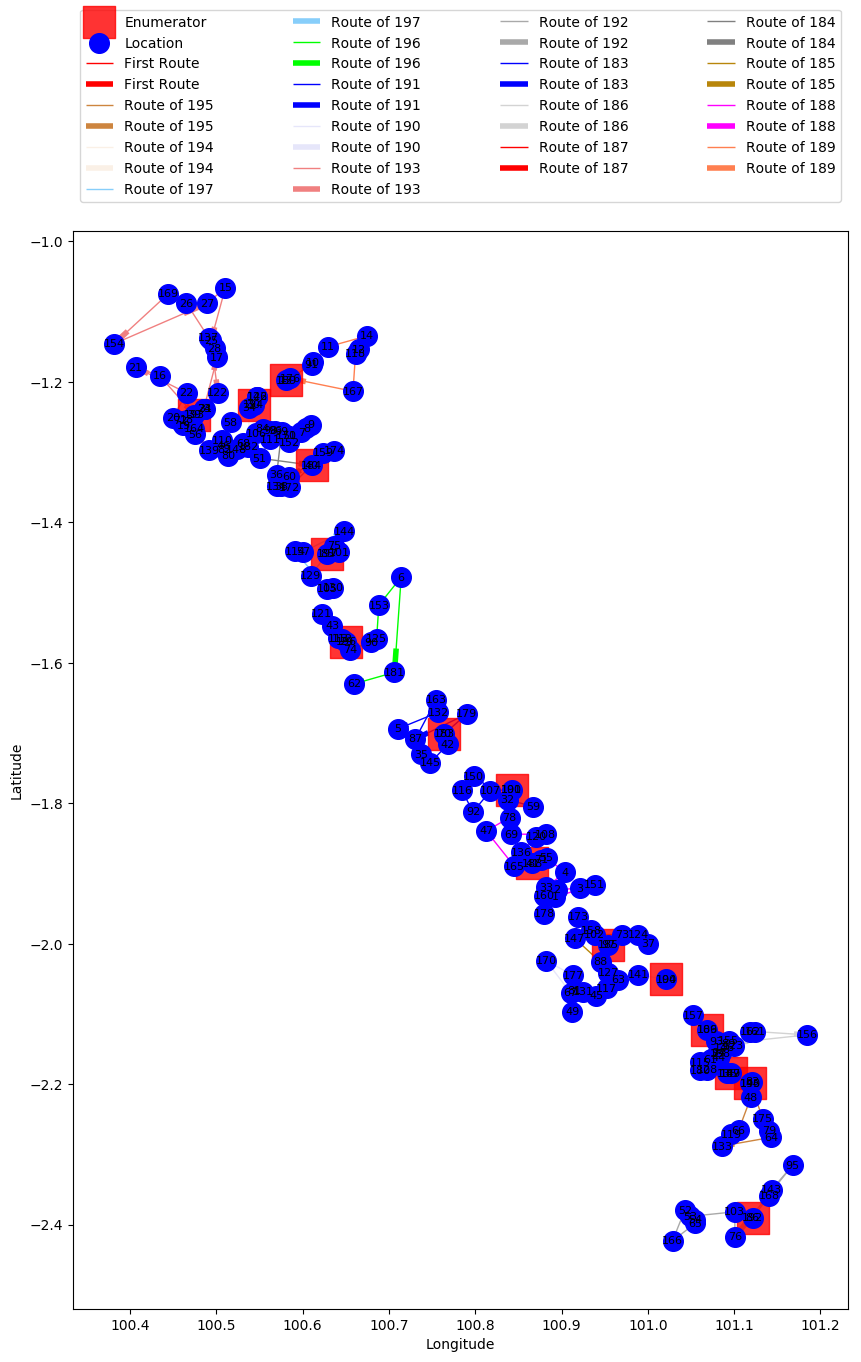
\includegraphics[width=\textwidth]{Resources/Images/test_result_normal_field_m15_n182_packet_loss_coes}
	\caption{Rute Hasil Pengujian Kondisi \textit{Packet Loss} Data Lapangan Pada MDVRP berbasis CoEAs}
	\label{fig:test_result_packet_loss_field_coes}
\end{figure}


\begin{figure}[H]
	\centering
	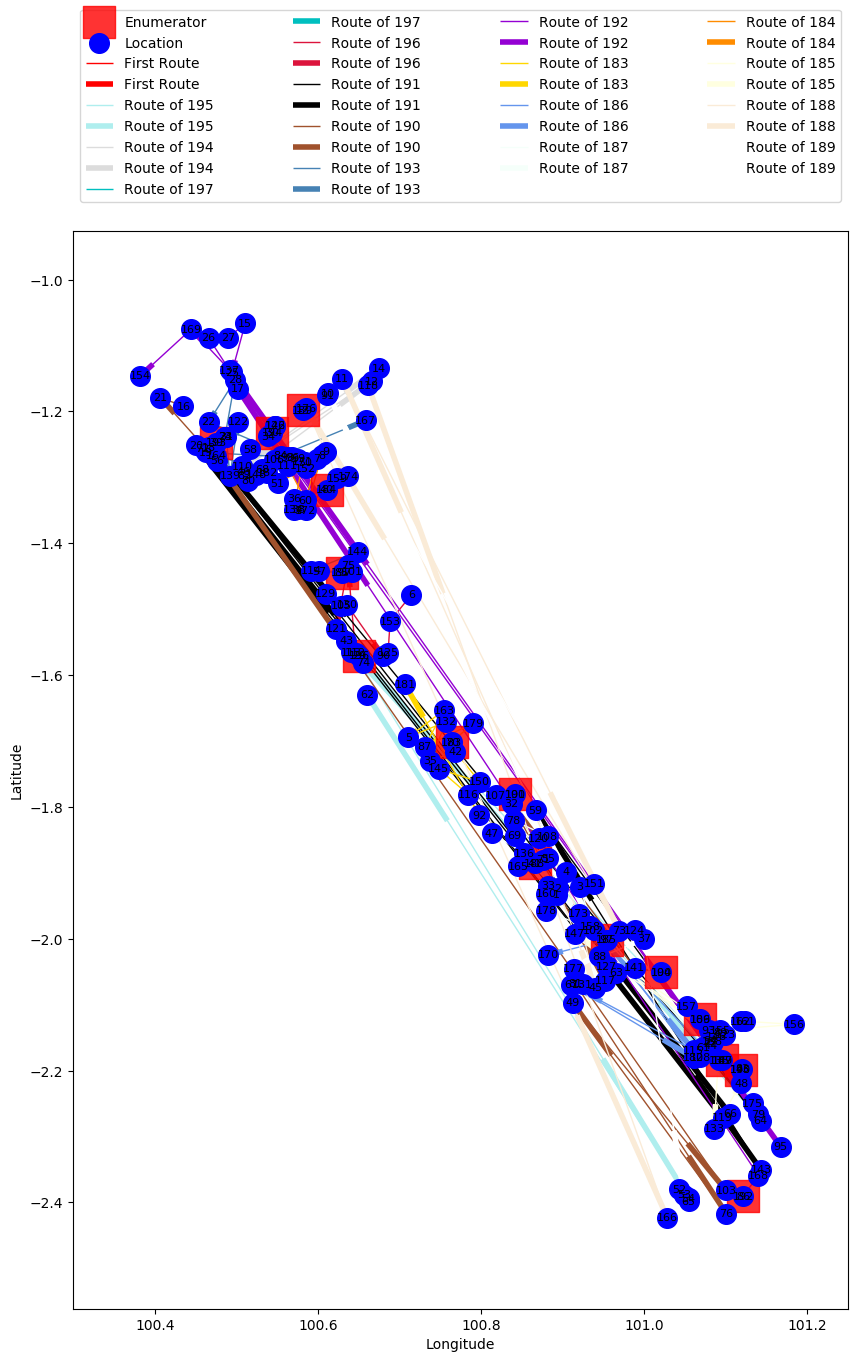
\includegraphics[width=\textwidth]{Resources/Images/test_result_normal_field_m15_n182_packet_loss_pubsub_coes}
	\caption{Rute Hasil Pengujian Kondisi \textit{Packet Loss} Data Lapangan Pada MDVRP berbasis CoEAs dengan Publish/Subscribe}
	\label{fig:test_result_packet_loss_field_pubsub_coes}
\end{figure}


%%-----------------------------------------------------------------------------%
%\subsubsection{Pengujian Kondisi Pencacah Berhenti}
%%-----------------------------------------------------------------------------%
%Skenario pengujian kondisi pencacah berhenti dimaksudkan untuk membandingkan program yang dijalankan pada kondisi dimana satu atau lebih pencacah berhenti pada saat pencacahan tengah berlangsung. Pengujian akan dilakukan satu kali untuk data lapangan. Pada pengujian ini sebuah program \textit{client} dirancang sebagai simulator.
%
%
%\begin{figure}[!]
%    \centering
%    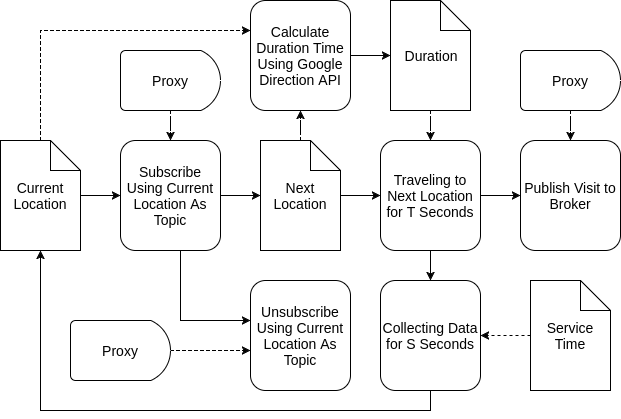
\includegraphics[width=\textwidth]{Resources/Images/client-algorithm-enumerator-quit-field}
%    \caption{\textit{Flowchart} pada \textit{Client Simulator} Kondisi Pencacah Berhenti}
%    \label{fig:client-algorithm-enumerator-quit-field}
%\end{figure}
%
%
%Langkah-langkah yang diimplementasikan pada program \textit{client}, sebagaimana ilustrasi Gambar \ref{fig:client-algorithm-enumerator-quit-field}, adalah sebagai berikut:
%
%\begin{enumerate}
%\item Buat koneksi dengan \textit{message broker}, 
%\item Lakukan \textit{subscription} dengan topik \textit{current location}, 
%\item Setelah sebuah \textit{message} diterima, dimana \textit{message} dari \textit{broker} merupakan \textit{next location}, kalkulasi waktu tempuh antara \textit{current location} dengan \textit{next location},
%\item Simulasikan perjalanan ke lokasi dengan \textit{sleep},
%\item Buat notifikasi terhadap broker atas perubahan \textit{current location}, 
%\item Generate \textit{service time}, mengikuti distribusi normal, 
%\item Simulasikan pencacahan dengan \textit{sleep}, 
%\item Hentikan beberapa proses, 
%\item Ulangi lagi dari langkah pertama.
%\end{enumerate}
%
%
%Pada pengujian ini, disimulasikan bahwasannya pencacah 1302110003 berhenti setelah 150000 detik, 1302101005 setelah 360000 detik, 1302012003 setelah 180000 detik, dan 1302080006 setelah 300000 detik. Tabel \ref{tbl:test_result_enumerator_quit_field_pubsub_coes} menunjukkan hasil simulasi dan waktu total untuk masing-masing pencacah. Ketika rute dari keempat pencacah tersebut dikeluarkan dari penghitungan standar deviasi, maka sebagaimana Tabel \ref{tbl:test_result_enumerator_quit_field} diperoleh .
%
%\begin{longtable}[!]{lp{8cm}r}
%	\caption{Hasil Pengujian Kondisi Pencacah Berhenti (Lapangan), CoEAs}
%	\label{tbl:test_result_enumerator_quit_field_coes}\\
%	\toprule
%		\textit{Vehicle} & Rute & Waktu Total\\ 
%	\midrule
%	\endfirsthead
%	\toprule
%		\textit{Vehicle} & Rute & Waktu Total\\ 
%	\midrule
%	\endhead
%	\bottomrule
%	\endfoot
%		
%\end{longtable}
%
%
%\begin{longtable}[!]{lp{8cm}r}
%	\caption{Hasil Pengujian Kondisi Pencacah Berhenti (Lapangan), CoEAs + Publish/Subscribe}
%	\label{tbl:test_result_enumerator_quit_field_pubsub_coes}\\
%	\toprule
%		\textit{Vehicle} & Rute & Waktu Total\\ 
%	\midrule
%	\endfirsthead
%	\toprule
%		\textit{Vehicle} & Rute & Waktu Total\\ 
%	\midrule
%	\endhead
%	\bottomrule
%	\endfoot
%		1302011008 & 1302011008-1302011008-1302011010-1302011001-1302012005-1302011007-1302011009-1302011005-1302011006-1302011002-1302011004-1302011003-1302090007-1302090015-1302110002-1302110013-1302110006 & 407401.10 \\
%		1302040002 & 1302040002-1302040002-1302040016-1302040004-1302040005-1302040006-1302040015-1302040007-1302040003-1302040009-1302040013-1302040008-1302090013 & 306233.49 \\
%		1302012003 & 1302012003-1302012008-1302012003-1302012001-1302012006-1302012002-1302012004-1302012010 & 169070.15 \\
%		1302060005 & 1302060005-1302060005-1302060009-1302060006-1302060008-1302060007-1302060001-1302060004-1302050010-1302050009-1302060003-1302012009-1302100016-1302090010 & 345013.89 \\
%		1302020006 & 1302020006-1302020006-1302020016-1302020015-1302021002-1302021006-1302020017-1302031005 & 171648.83 \\
%		1302080006 & 1302080006-1302080006-1302080007-1302080008-1302080002-1302080001-1302080004-1302080009-1302070012-1302070003-1302080003-1302080005 & 269836.91 \\
%		1302021005 & 1302021005-1302021005-1302021001-1302020011-1302020009-1302020001-1302020010-1302021003-1302021008-1302021010-1302021007-1302021009-1302021004-1302110012 & 335580.21 \\
%		1302100002 & 1302100002-1302100002-1302100003-1302100013-1302100009-1302100001-1302100005-1302110023-1302110021-1302110022-1302110008-1302110007-1302110020-1302110018-1302110009-1302110003-1302110010-1302110005 & 428783.15 \\
%		1302101005 & 1302101005-1302101005-1302100010-1302101002-1302100014-1302100011-1302101003-1302101001-1302100006-1302100004-1302100012-1302100007-1302100017-1302101004 & 327886.72 \\
%		1302110003 & 1302110003-1302110019-1302110004-1302110001-1302110011-1302110017-1302110016 & 147061.67 \\
%		1302090004 & 1302090004-1302090008-1302090002-1302090005-1302090004-1302090012-1302090014-1302090020-1302090019-1302090001-1302090017-1302090018-1302090016-1302110014-1302101006-1302090011 & 368625.31 \\
%		1302030005 & 1302030005-1302030005-1302030014-1302030006-1302030009-1302030004-1302030012-1302030003-1302031004-1302030010-1302030002-1302031003-1302020005-1302020003-1302100015-1302100008 & 382133.70 \\
%		1302070006 & 1302070006-1302070006-1302070002-1302070011-1302070005-1302070008-1302070009-1302070010-1302070007-1302070001-1302070004-1302060002-1302110015 & 299606.48 \\
%		1302050007 & 1302050007-1302050007-1302050008-1302050002-1302050006-1302050004-1302050001-1302050003-1302050005-1302040001-1302040012-1302012007-1302090006-1302090009-1302090003 & 369932.48 \\
%		1302031005 & 1302031005-1302031001-1302031006-1302031008-1302040011-1302031009-1302031010-1302040010-1302031007-1302030001-1302031002-1302040014 & 278953.18 \\
%\end{longtable}
%
%
%\begin{longtable}[!]{lrr}
%	\caption{Komparasi CoEAs dan Publish/Subscribe + CoEAs pada Data Lapangan}
%	\label{tbl:test_result_enumerator_quit_field}\\
%	\toprule
%		Ukuran & CoEAs & CoEAs + Publish/Subscribe\\ 
%	\midrule
%	\endfirsthead
%	\toprule
%		Ukuran & CoEAs & CoEAs + Publish/Subscribe\\ 
%	\midrule
%	\endhead
%	\bottomrule
%	\endfoot
%		Total Waktu & 4448989.67 & 4607767.28\\
%		Rata-rata & 296599.31 & 307184.49\\
%		Standar Deviasi & 119720.84 & 84126.97\\
%\end{longtable}

